\documentclass[11pt,a4paper]{article}
\usepackage[utf8]{inputenc}
\usepackage[T1]{fontenc}
\usepackage{lmodern}
\usepackage[margin=2.5cm]{geometry}
\usepackage{amsmath,amssymb}
\usepackage{booktabs}
\usepackage{graphicx}
\usepackage{xcolor}
\usepackage{url}
\usepackage[colorlinks=true,linkcolor=blue!50!black,citecolor=blue!50!black,urlcolor=blue!50!black]{hyperref}

\newcommand{\R}{\mathbb{R}}
\DeclareMathOperator{\sgn}{sgn}

\title{Exact exponential rates for the discrete Calder\'on problem on lattice strips:\\ and what transient data do not change}
\author{Xavier Callens\\[2pt]
\small SocrateAI Lab, Cagnes-sur-Mer, France\\
\small \texttt{callensxavier@gmail.com}}
\date{October 2026 \\ \small Preprint, not peer reviewed. Companion to the preprint doi:10.5281/zenodo.23228685}

\begin{document}
\maketitle

\begin{abstract}
Exponential ill-conditioning of the inverse conductivity problem, and of its discrete network versions, is classical. The
preprint cited above measured the condition number of the Jacobian of the Dirichlet-to-Neumann (DtN) map of a resistor network
with respect to its edge conductances, and found exponential growth with the depth of the unknowns on flat lattice disks and
polynomial growth on hyperbolic tilings. Here we only add a sharp exponent on a solvable family:
a lattice strip, periodic along a boundary row that carries the measurements. Translation invariance makes the Jacobian
exactly block-diagonal in the total momentum along the boundary; each block is a Vandermonde-type matrix whose nodes are the
products of the per-row decay factors of two boundary modes. The smallest singular value of block $q$ then decays with depth
at the exponent $G(q)$ of the Green function of the complement of the node set, evaluated on the unit circle, and the global
rate is attained at the zigzag momentum $q=\pi$. We check this in 140- to 220-digit arithmetic: for the aligned square strip
with unit conductances the zigzag rate is $1.653$ decades per row, for a boundary along the lattice diagonal it is $1.067$,
and for lateral-to-vertical conductance ratios $0.05$ and $16$ it is $1.762$ and $2.498$ (predicted $1.765$ and $2.451$,
fixed before the computation), non-monotone in the ratio; at converged width all momenta agree with the prediction to within
$2\,\%$. A further preregistered experiment asks whether transient data, represented by real Laplace variables, change the depth growth of the condition number on a square disk: they lower it by about one decade and leave the exponential rate unchanged (post hoc slope ratio $0.98$). Four elementary linear-algebra facts behind the offset-invisibility of the measurement are machine-checked in Lean 4. The note records its failures: two closed forms of mine were wrong (one preregistered), the diagonal case needed a
sign correction that was found after the data, and three design errors (finite reference height, depth windows, tolerances)
are kept in a register. The exponent is an asymptotic statement for many nodes, argued by a Bernstein--Walsh sketch, not proved. Closely related rigorous
results exist for real nodes and for Hankel matrices, and we have not established that the exact statement is new. The disk,
curvature, and complex node sets are open. Nothing here concerns holography.
\end{abstract}

\section{Setting}
A resistor network has nodes, edges $e$ with conductances $g_e>0$, and a set of $m$ boundary nodes where voltages are imposed
and currents measured; recovering the conductances from these data is the discrete Calder\'on problem~\cite{Calderon,CurtisMorrow}.
The empirical background is the companion preprint~\cite{Preprint}.
\emph{Related work.} Exponential instability of the continuous problem is established~\cite{DiCristoRondi}, and for discrete network
recovery the conditioning is known to degrade exponentially with the number of boundary nodes or layers~\cite{BorceaReview,BorceaNoise};
for layered networks the problem reduces to Fourier blocks and a Vandermonde-type inversion~\cite{BorceaReview}, and a numerical study
of exponential growth with slice index on lattices states the rigorous analysis as open~\cite{DengJin}. Exponential lower bounds for Vandermonde
matrices with real nodes go back to Gautschi~\cite{Gautschi62,Gautschi75}; sharp real-node rates are due to Beckermann (Numer.\ Math.\ 85, 2000),
and a lower bound for complex nodes through the nodal polynomial on the unit circle to Pan~\cite{Pan}. The smallest eigenvalue of Hankel
matrices decays exponentially for compactly supported measures~\cite{BergSzwarc}, with sharp rates going back to Szeg\H{o} (1936) and
Widom and Wilf (1966), which we have not read. The Green-function duality we use is the one that governs stable analytic extrapolation~\cite{DemanetTownsend}.
We have found no source that states the rate as the maximum over the unit circle of the Green function of the complement of a complex node set,
but our search was limited. Hyperbolic lattices have been built as circuits~\cite{Lenggenhager}; we are not aware of work on the
conditioning of the inverse conductance problem on them. The DtN map $\Lambda(g)\in\R^{m\times m}$ is the Schur complement of the weighted graph Laplacian onto
the boundary. By the envelope theorem the derivative of $\Lambda$ with respect to the conductance of edge $e=(a,b)$ is
$\partial\Lambda/\partial g_e=d_e d_e^{\top}$, where $d_e=H_a-H_b\in\R^m$ is the difference of the rows of the harmonic extension
$H$ (boundary data $\mapsto$ node potentials) at the endpoints of $e$. Collecting the strictly upper-triangular entries of
$\partial\Lambda/\partial g_e$ as the column of $e$ gives the Jacobian $J$ used throughout (the diagonal of $\Lambda$ is
determined by its row sums). The \emph{depth} of an edge is the smaller of the graph distances of its endpoints to the
boundary, and $J_d$ is $J$ restricted to the columns of depth $\le d$. We study $\kappa(J_d)=\sigma_{\max}/\sigma_{\min}$ as a
function of $d$; the companion preprint reports $\log_{10}\kappa(J_d)$ growing roughly linearly with $d$ on flat disks.

The solvable family is the \emph{strip}: nodes $(s,j)$, $s=0,1,2,\dots$ (rows, $s=0$ the boundary), $j\in\mathbb Z_W$
(periodic along the boundary), semi-infinite in $s$. We treat two orientations of the square lattice relative to the
boundary. In the \emph{aligned} strip, node $(s,j)$ is joined to $(s,j\pm1)$ with conductance $\lambda$ and to $(s\pm1,j)$ with
conductance $1$. In the \emph{diagonal} strip (the lattice rotated by $45^\circ$ with respect to the boundary, periodic along
$(1,1)$), the rows are $s=x-y$ and each node of row $s$ is joined to the nodes $j$ and $j+1$ of row $s+1$, with no edges inside a
row; the graph depth is then the $L^1$ distance to the boundary.

\section{Block structure}
Translation $j\mapsto j+1$ acts on the edges and, compatibly, on the data (the strictly upper-triangular entries), and
$J$ intertwines the two actions. Fourier transforming the columns over the position $j$ of the edge therefore makes $J$ exactly
block-diagonal in the total momentum $q=2\pi i/W$, $i\in\mathbb Z_W$ (I checked numerically that the union of the block
singular values equals the spectrum of the unblocked matrix to $2\times10^{-15}$).

\paragraph{Aligned strip.} A boundary mode $e^{ikj}$ has the harmonic extension $z_1(k)^s e^{ikj}$ with
$z_1=e^{-\kappa(k)}$ and $\cosh\kappa(k)=1+\lambda(1-\cos k)$. A vertical edge at depth $r$ has signature
$d_e\propto z_1(k)^r(1-z_1(k))$ per mode, so for the vertical-edge columns the block at momentum $q$ is
\begin{equation}
V_q[n,r]=a_n z_n^{\,r},\qquad z_n=z_1(k_n)\,z_1(q-k_n),\quad a_n=\bigl(1-z_1(k_n)\bigr)\bigl(1-z_1(q-k_n)\bigr),\quad k_n=\tfrac{2\pi n}{W},
\label{eq:block}
\end{equation}
with rows $n$ indexing the pair of modes $(k_n,q-k_n)$ and columns $r=0,\dots,d$ the depths. Because the data exclude the
diagonal of $\Lambda$, the position-diagonal direction, which in the block is the uniform vector over $n$, is projected out:
$V_q\mapsto(I-uu^{\top})V_q$, $u=\mathbf 1/\sqrt W$. Without this projection the block does not reproduce the explicit
Jacobian; with it the exact block agrees with the explicit double-precision block at large height to $0.005$ decades in every
per-row increment.

\paragraph{Diagonal strip.} The decay factor $\lambda(k)$ of the mode $e^{ikj}$ is the root with $|\lambda|<1$ of
$(1+e^{ik})\lambda^2-4\lambda+(1+e^{-ik})=0$; $|\lambda(k)|=\rho(k)=(1-\sin(|k|/2))/\cos(k/2)$ and the zigzag mode $k=\pi$
decouples ($\lambda=0$). The block of the edges joining $(s,j)$ to $(s+1,j)$ has the form~\eqref{eq:block} with
$z_n=\lambda(k_n)\lambda(q-k_n)$, $a_n=(1-\lambda(k_n))(1-\lambda(q-k_n))$.

\section{The rate}\label{sec:rate}
Let $K_q\subset\mathbb C$ be the set of node values $\{z_n\}$ of block $q$. The geometric growth of the condition number of
Vandermonde matrices is classical~\cite{Gautschi62,Gautschi75}; what is needed here is its exact rate for the node sets that
arise. For a polynomial $p(z)=\sum_{r\le d}c_rz^r$ the
vector $V_qc$ has entries $a_np(z_n)$, so $\sigma_{\min}(V_q^{(d)})$ is governed by how small $p$ can be on $K_q$ relative to the
coefficient norm $\|c\|_2$. The Bernstein--Walsh inequality, $|p(\zeta)|\le\|p\|_{K}\,e^{d\,g_K(\zeta)}$ with $g_K$ the Green function
of the complement of $K$ with pole at infinity~\cite{Ransford,SaffTotik}, gives, with $|c_r|\le\max_{|\zeta|=1}|p|$,
\[
\|c\|_2\le\sqrt{d+1}\;\|p\|_{K}\,e^{d\,G},\qquad G=\max_{|\zeta|=1}g_K(\zeta),
\]
hence a lower bound $\sigma_{\min}\gtrsim e^{-dG}$ up to subexponential factors. For a regular compact set the bound is
attained up to subexponential factors by Chebyshev-type polynomials (the standard extremal theory~\cite{SaffTotik}), and the
weights $a_n$ and the one-direction projection only enter the subexponential factors. We use this as the \emph{prediction}
\begin{equation}
\sigma_{\min}\bigl(V_q^{(d)}\bigr)\approx 10^{-G(q)\,d},\qquad G(q)=\frac{1}{\ln 10}\max_{|\zeta|=1}g_{K_q}(\zeta),
\label{eq:rate}
\end{equation}
and test it numerically; we do not claim a proof. When $K_q$ is a real interval $[a,b]$,
$g(\zeta)=\log\bigl|w+\sqrt{w^2-1}\bigr|$ with $w=(2\zeta-a-b)/(b-a)$ (branch of modulus $>1$), and in every case below the
maximum over the circle is attained at $\zeta=-1$. Since $\sigma_{\max}$ is attained at the shallow columns and varies
only polynomially with $d$, the condition number grows at the largest $G(q)$, which is attained at the zigzag momentum $q=\pi$:
the block with the smallest top node, not the one with the widest spread of nodes. (My first estimate of the rate used the
Chebyshev growth of $[a,1]$ after rescaling by $z_{\max}$ and evaluated it at the wrong point; it predicted $1.833$ for the
aligned strip and was wrong, Section~\ref{sec:failures}.)

A finite boundary carries finitely many data per momentum: at $q=\pi$ and $W$ sites the block has only $W/4+1$ distinct nodes
(the values are invariant under $k\mapsto-k$ and $k\mapsto\pi-k$), so $J_d$ is rank-deficient beyond a depth set by $W$, and
at depths comparable to the number of distinct nodes the measured per-row loss drifts upward from $G$. We therefore take rates
over depths $15$--$25$ at $W=384$ ($97$ distinct nodes at $q=\pi$) and check the zigzag block again at $W=768$.

\section{Verification}\label{sec:verify}
\paragraph{Method.} The blocks~\eqref{eq:block} are built in 140 digits (220 for the large-ratio case), and
$\sigma_{\min}$ of the first $d+1$ columns is computed as $1/\sqrt{\lambda_{\max}(G^{-1})}$, $G=V^{\dagger}V$, by power iteration
(the spectrum of $G^{-1}$ is geometric, so a few iterations suffice). The validity gate compares the exact zigzag block with the
explicit double-precision block of the Jacobian of a $W=96$ cylinder of large height, for the per-row increments at $d\le5$.

\paragraph{Result.} Table~\ref{tab:rates} and Figure~\ref{fig:rates} compare measured and predicted rates for six momenta in
four geometries. For the aligned strip with $\lambda=1$ the zigzag rate is $1.653$ at $W=768$ (prediction $1.653$) and the six
momenta agree to $0.06$--$1.6\,\%$ at $W=384$. For the aligned strip with $\lambda=0.05$ and $16$, whose predictions
($1.765$ and $2.451$ for the zigzag block, and the five other momenta) were fixed before the computation and which have a
different dispersion relation, the converged zigzag rates are $1.762$ and $2.498$; for $\lambda=0.05$ all six momenta are
within $0.7\,\%$, for $\lambda=16$ the five non-zigzag momenta are within $2.2\,\%$ (all on the high side) and the zigzag block at
$W=384$ overshoots by $8\,\%$ because its per-row loss still drifts with depth (Figure~\ref{fig:inc}) when only 97 distinct nodes
are available; at $W=768$ the overshoot is $1.9\,\%$. The zigzag momentum carries the smallest $\sigma_{\min}$ at depth $20$ in
every case. The null hypothesis that the rate does not depend on $\lambda$ is refuted by $6.6\,\%$ and $51\,\%$.

% GENERATED by make_note_cylinder.py from data/*.json -- do not edit
\begin{table}[t]\centering\scriptsize
\caption{Measured / predicted decay rate of $\sigma_{\min}$ (decades per row) of the momentum blocks, exact semi-infinite computation at $W=384$ (last column: zigzag block at $W=768$). Predictions are the Green-function exponents of the node sets; for the diagonal boundary the signed-node form was found after the data (Section~\ref{sec:orient}), the moduli-only form was the preregistered one.}
\label{tab:rates}
\resizebox{\linewidth}{!}{%
\begin{tabular}{lccccccc}\toprule
Geometry & $\pi/6$ & $\pi/3$ & $\pi/2$ & $2\pi/3$ & $5\pi/6$ & $\pi$ & $\pi$ ($W{=}768$) \\ \midrule
aligned, $\lambda=1$ & 0.955 / 0.961 & 1.133 / 1.138 & 1.295 / 1.298 & 1.436 / 1.435 & 1.554 / 1.551 & 1.679 / 1.653 & 1.653 / 1.653 \\
diagonal (signed nodes) & 0.838 / 0.846 & 0.917 / 0.922 & 0.985 / 0.991 & 1.039 / 1.044 & 1.065 / 1.071 & 1.067 / 1.070 & 1.067 / 1.070 \\
aligned, $\lambda=0.05$ & 1.135 / 1.141 & 1.227 / 1.233 & 1.334 / 1.339 & 1.457 / 1.461 & 1.599 / 1.601 & 1.777 / 1.765 & 1.762 / 1.765 \\
aligned, $\lambda=16$ & 1.440 / 1.423 & 1.900 / 1.870 & 2.186 / 2.144 & 2.366 / 2.314 & 2.460 / 2.411 & 2.647 / 2.450 & 2.497 / 2.450 \\
diagonal, moduli only (wrong) & 0.838 / 0.849 & 0.917 / 0.938 & 0.985 / 1.036 & 1.039 / 1.144 & 1.065 / 1.265 & 1.067 / 1.403 & 1.067 / 1.403 \\
\bottomrule\end{tabular}}\end{table}

\begin{table}[t]\centering\scriptsize
\caption{Register of the preregistered gates and predictions behind this note, from the stored verdicts. Every refutation is kept; the failed gates are design errors of mine (Section~\ref{sec:failures}).}
\label{tab:register}
\begin{tabular}{llp{3.2cm}p{5.6cm}}\toprule
Prereg. & Ledger & Gates & Predictions \\ \midrule
23 & H0-X-0014 & G1 pass, G2 pass, G3 fail & P1 refuted, P2 held, P3 refuted, P4 void \\
24 & H0-X-0015 & G1 pass, G2 fail & P1 held, P2 refuted, P3 held \\
25 & H0-X-0016 & G1 pass & P1 held, P2 held, P3 held, P4 refuted, P5 held \\
26 & H0-X-0017 & G1 pass & P1 refuted, P2 refuted, P3 held, P4 held \\
27 & H0-X-0018 & G1 fail & P1 held, P2 refuted, P3 held, P4 refuted, P5 held \\
\bottomrule\end{tabular}\end{table}


\begin{figure}[t]
\centering
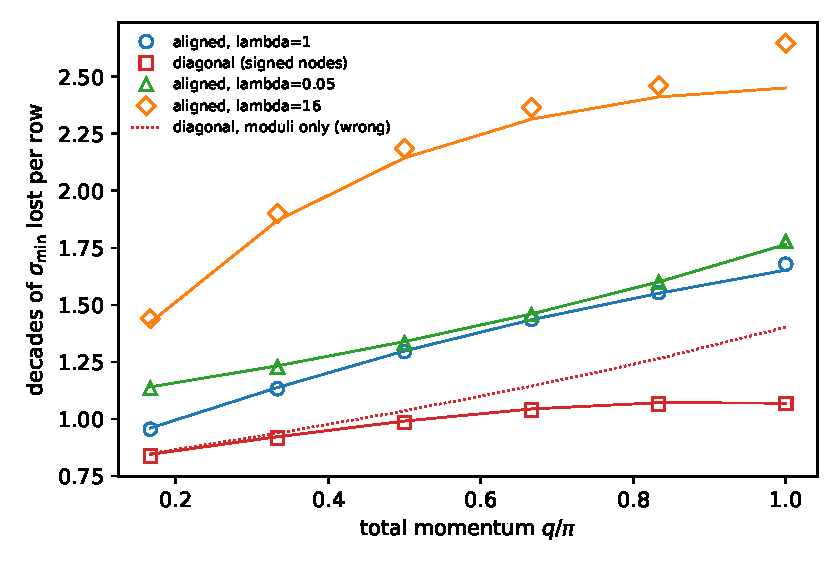
\includegraphics[width=0.78\linewidth]{fig_note_rates.pdf}
\caption{Decay rate of $\sigma_{\min}$ against total momentum, $W=384$: markers measured, lines predicted (Green exponent of the node
set). The dotted red line is the preregistered but wrong prediction for the diagonal boundary (moduli of the nodes only).}
\label{fig:rates}
\end{figure}

\begin{figure}[t]
\centering
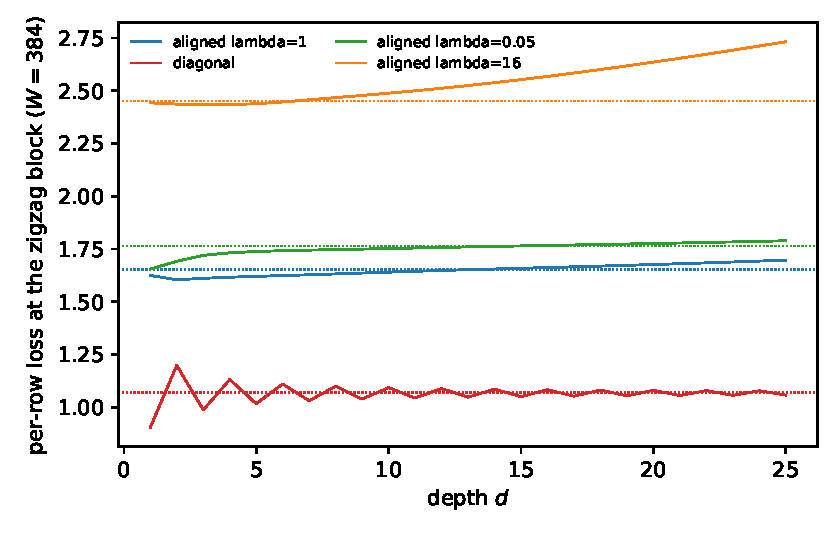
\includegraphics[width=0.78\linewidth]{fig_note_increments.pdf}
\caption{Per-row loss of $\sigma_{\min}$ at the zigzag block against depth, $W=384$ (dotted: prediction). The aligned $\lambda=16$
curve drifts upward with depth (too few distinct nodes at this decay rate); the diagonal curve alternates with period two,
the signature of nodes of both signs (Section~\ref{sec:orient}).}
\label{fig:inc}
\end{figure}

\section{Orientation and signed nodes}\label{sec:orient}
For the diagonal strip the exact blocks (gate agreement to $0.001$) give the zigzag rate $1.067$ decades per row, 35\,\% below
the aligned value, and the same zigzag dominance. Two preregistered forms for this rate were wrong: the Green exponent of the
\emph{moduli} of the nodes ($1.403$) and the geometric guess that the rate per graph step is the aligned rate divided by
$\sqrt2$, because graph depth is the $L^1$ distance ($1.169$). The per-row increments printed by the computation alternated
with period two. That led to the explanation, \emph{found after the data}: after removing the common phase $e^{-iq/2}$ the
node values $\lambda(k)\lambda(q-k)$ are real (imaginary parts $10^{-16}$) but of both signs, because the sign flips when $q-k$
wraps around $2\pi$. The node set is then the single interval $[-M_-,M_+]$ through zero, and its Green exponent
reproduces all six measured rates to between $0.2\,\%$ and $0.85\,\%$ with no free parameter (Table~\ref{tab:rates}). Because this
was fitted to the data it is a hypothesis for the diagonal strip, supported by agreement on six numbers; the aligned family of the
previous section is the independent test of the underlying picture. For unequal conductances on the two edge types of the diagonal
strip the nodes are genuinely complex (imaginary parts up to $0.16$ against moduli up to $0.2$), and the interval formula does
not apply.


\section{Transient data}\label{sec:laplace}
The hardware that motivates the companion preprint is read with a scope, so its data are transients and not only the direct-current response matrix.
For a step response of the resistor--capacitor network (unit conductances, unit capacitance from each interior node to ground) the Laplace transform of
the boundary current gives the response matrix $\Lambda(s)=L_{bb}-L_{bi}(L_{ii}+sI)^{-1}L_{ib}$ at real $s$, and the same envelope argument as at $s=0$ gives
$\partial\Lambda(s)/\partial g_e=d_e(s)d_e(s)^{\top}$ with $d_e(s)$ the difference of the rows of $-(L_{ii}+sI)^{-1}L_{ib}$ at the endpoints of $e$. Stacking the Jacobians
over a set $S$ of Laplace variables gives $J_d(S)$; since $J_d(S)^{\top}J_d(S)\ge J_d(0)^{\top}J_d(0)$, the smallest singular value can only rise
(an exact consequence, gate G2, which held). Whether the condition number's exponential growth with depth is slowed is not implied, and preregistration 29 asked it before the run.

The link between time and frequency was checked with the CVODE integrator of rusty-SUNDIALS (BDF, relative tolerance $10^{-10}$): the Laplace transform of the integrated boundary current
must equal $\Lambda(s)e_j/s$ to $10^{-5}$. As written this gate \emph{failed} at $s=0.1$ (relative error $1.6\times10^{-3}$): the held step leaves a nonzero steady current, and my
integration window ended where $e^{-sT}/s$ was still $10^{-3}$ of the integral. A tail term from the integrator's own final current repairs it (errors between $10^{-14}$ and $4\times10^{-10}$ at $s=0.1,0.3,1$),
but this variant was declared after the failure and is post hoc.

\paragraph{Result.} On the square disk of radius 16 the stacked condition number is lower by about one decade at every depth with five Laplace variables
(Table~\ref{tab:laplace}), while the growth rate is unchanged. The preregistered prediction that the five-variable slope would not exceed the direct-current slope was
\emph{refuted}, narrowly: the preregistered window, restricted by a double-precision floor to $d=3,4$, gave a ratio of $1.025$ from two points. Over $d=3,\dots,9$ (post hoc) the slopes
are $1.175$, $1.123$ and $1.155$ decades per step for one, two and five variables. On the $\{7,3\}$ tiling with four layers the condition number changes by a quarter of a decade.
For the board this means that sampling the transient is worth about one decade of conditioning and does not alter the conclusion that deep edges are exponentially harder to see.
Limits: double precision, noise-free, real $s$ only, one disk size, and the condition number of a stacked matrix as the figure of merit.

\section{Machine-checked linear algebra}\label{sec:lean}
Four elementary facts behind the invisibility of constant offsets are formalised in Lean 4 against Mathlib (files in the repository under \texttt{lean/dtn\_offsets}): a matrix with zero row sums and an invertible
interior block has a Schur complement with zero row sums; a matrix with zero row sums is Frobenius-orthogonal to any offset constant along rows, and dually for columns given zero column sums;
and an additive disturbance orthogonal to two candidate signatures leaves the difference of their squared distances to the data unchanged. The build, the search for \texttt{sorry}, the axiom audit
(each theorem depends only on \texttt{propext}, \texttt{Classical.choice}, \texttt{Quot.sound}) and a statement lock pass, and a separate agent audited the wording, which led to three docstring corrections.
These lemmas are elementary; they say nothing about conditioning, geometry or holography, and the identification of the Jacobian columns with the objects in them is not formalised.

\section{What failed}\label{sec:failures}
Every preregistered gate and prediction is kept (Table~\ref{tab:register}); four of the eleven evaluable predictions of the first three
cards were refuted and one was void, and later cards added more. The errors, all mine, in order:
(i) the preregistered rate $0.784$ for the aligned strip was a single-block estimate and the measurement was $1.78$ at finite height;
(ii) the corrected closed form $1.833$, derived after seeing that number, agreed with a finite-height window average to $3\,\%$
and was wrong (the exact value is $1.653$); (iii) double-precision data at a finite cylinder height are contaminated by the closed
end at the level of tenths of a decade, and the per-row increments were still rising there; a reference gate of height $40$
failed at weak lateral coupling, where the explicit increments converge to the exact ones only at height $160$; (iv) a depth window
of $20$--$30$ at $W=96$ is impossible because the block has $25$ distinct nodes; (v) width-convergence tolerances were too tight for
fast decay; (vi) the straight periodic triangular boundary row has an exact null vector of the Jacobian at depth $0$ (translation
invariance plus mirror symmetry), so no triangular value could be obtained on that geometry. (vii) in the transient experiment, the integration window of the time-to-frequency gate ignored the steady current (Section~\ref{sec:laplace}), and the double-precision floor shrank the preregistered depth window to two points. These are recorded as lessons
in the repository's lesson file.

\section{Limits and open questions}
All results are computations on the semi-infinite strip with unit or two-valued conductances; the Bernstein--Walsh bound is a
sketch, not a proof of the rate. The square disk measured in the companion work loses about $1.1$--$1.2$ decades per graph
step, below the aligned strip's $1.65$; a disk combines all boundary orientations with curvature and a staircase boundary,
and nothing here says how they combine. The hyperbolic tilings, whose boundary grows with depth, are not covered, nor are
triangular lattices with a generic boundary or complex node sets. The finite-height double-precision rates of earlier work
should not be read as rates of the semi-infinite problem. The Green-function exponent describes the regime where the number
of distinct nodes exceeds the depth (here 25 to 193 nodes against depths up to 25 rows); for a square system with about as many nodes as the degree the
exponent is a discrete nodal quantity instead. A separate preregistered run (preregistration 28, in the repository, not tabulated here) found on a polar-grid disk that curvature of this kind \emph{raises} the per-row loss with depth, so curvature does not explain the square disk's lower constant; boundary roughness and orientation mixture remain. The note does not concern holography, AdS/CFT or any physical
analogue.

\section*{Reproducibility}
Scripts \texttt{exp23}--\texttt{exp27}, \texttt{exp29} and their preregistrations \texttt{PREREGISTRATION\_23}--\texttt{27}, \texttt{29}, the data files under
\texttt{data/}, the ledger claims H0-X-0014 to H0-X-0018 with evidence digests (preregistration 29 is recorded in the results file but not entered in the ledger), and the post-hoc diagnostics (labelled as such) are in
the repository of the companion preprint (Zenodo concept DOI 10.5281/zenodo.23000390). The Lean files are in \texttt{lean/dtn\_offsets}. Every table and figure of this note is generated
from those data files by \texttt{paper/make\_note\_cylinder.py}.

\section*{Use of AI tools}
Code, numerical experiments and drafting were carried out with the assistance of Claude (Anthropic); the claims of the later
preregistered runs were recorded by a smaller model and audited against the data files by a larger one, following a written
runbook in the repository. The author directed the work and takes responsibility for the content.

\begin{thebibliography}{99}
\bibitem{Calderon} A.~P. Calder\'on, On an inverse boundary value problem, in \emph{Seminar on Numerical Analysis and its
Applications to Continuum Physics}, Soc.\ Brasil.\ Mat., 1980, pp.~65--73.
\bibitem{CurtisMorrow} E.~B. Curtis and J.~A. Morrow, \emph{Inverse Problems for Electrical Networks}, World Scientific, 2000.
\bibitem{Ransford} T.~Ransford, \emph{Potential Theory in the Complex Plane}, Cambridge University Press, 1995.
\bibitem{SaffTotik} E.~B. Saff and V.~Totik, \emph{Logarithmic Potentials with External Fields}, Springer, 1997.
\bibitem{Gautschi62} W.~Gautschi, On inverses of Vandermonde and confluent Vandermonde matrices, \emph{Numer.\ Math.} 4 (1962) 117--123.
\bibitem{Gautschi75} W.~Gautschi, Norm estimates for inverses of Vandermonde matrices, \emph{Numer.\ Math.} 23 (1975) 337--347.
\bibitem{DiCristoRondi} M.~Di Cristo and L.~Rondi, Examples of exponential instability for elliptic inverse problems, arXiv:math/0303126 (2003).
\bibitem{BorceaReview} L.~Borcea, V.~Druskin, F.~Guevara Vasquez and A.~V.~Mamonov, Resistor network approaches to electrical impedance tomography,
in \emph{Inside Out II}, MSRI Publications 60 (2012); arXiv:1107.0343.
\bibitem{BorceaNoise} L.~Borcea, F.~Guevara Vasquez and A.~V.~Mamonov, Study of noise effects in electrical impedance tomography with resistor networks,
\emph{Inverse Probl.\ Imaging} 7 (2013) 417--443; arXiv:1105.1183.
\bibitem{DengJin} M.~Deng and B.~Jin, On the uniqueness of the discrete Calder\'on problem on multi-dimensional lattices, arXiv:2509.18203 (2025).
\bibitem{Pan} V.~Y.~Pan, How bad are Vandermonde matrices?, \emph{SIAM J. Matrix Anal. Appl.} 37 (2016) 676--694; arXiv:1504.02118.
\bibitem{BergSzwarc} C.~Berg and R.~Szwarc, The smallest eigenvalue of Hankel matrices, \emph{Constr.\ Approx.} 34 (2011) 107--133.
\bibitem{DemanetTownsend} L.~Demanet and A.~Townsend, Stable extrapolation of analytic functions, arXiv:1605.09601 (2016).
\bibitem{Lenggenhager} P.~M.~Lenggenhager et al., Simulating hyperbolic space on a circuit board, \emph{Nat.\ Commun.} 13 (2022) 4373.
\bibitem{Preprint} X.~Callens, Logarithmic boundary depth and the conditioning of the discrete inverse conductance problem on hyperbolic
lattices (version 1.2), Zenodo, doi:10.5281/zenodo.23228685.
\end{thebibliography}
\end{document}
